\begin{figure}[H]
\centering
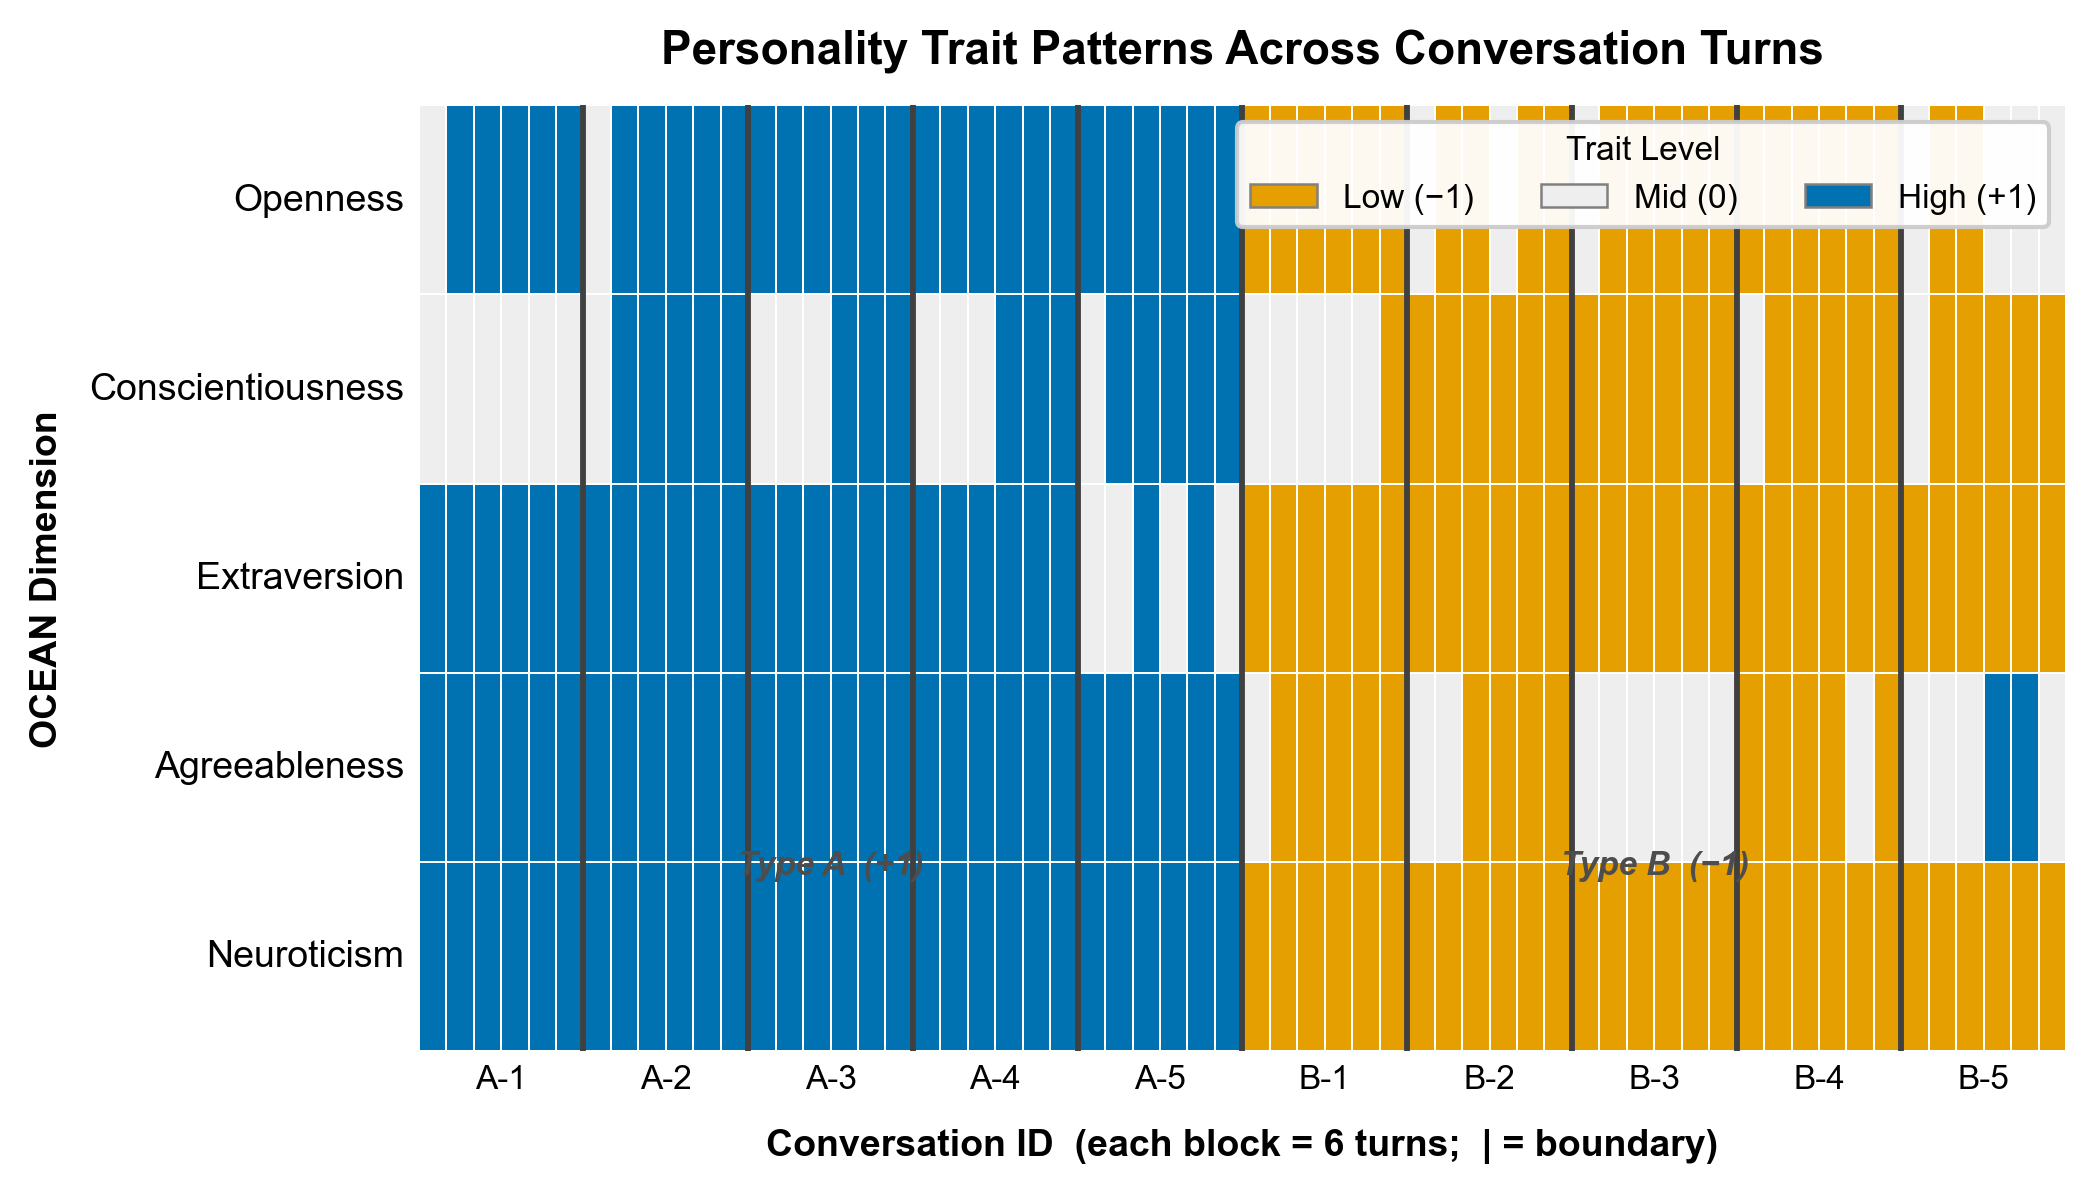
\includegraphics{figures/07_personality_heatmap.png}
\caption{Personality trait patterns across conversation turns (Regulated condition, $N = 60$ turns, sorted by Conversation ID). Each column represents one turn; each row represents one OCEAN dimension. Colors indicate trait levels: Blue = High ($+1$), Orange = Low ($-1$), Gray = Mid ($0$). Vertical lines mark conversation boundaries (each block = 6 turns). A broad color split is visible between the left (Type A) and right (Type B) halves, with blue dominant in Type A and orange dominant in Type B for most dimensions. Gray (Mid) patterns are more pronounced in Conscientiousness and Agreeableness, reflecting dimensions where neutral-state detection occurs more frequently even under extreme profile conditions.}
\label{fig:10}
\end{figure}
